\chapter{Background on Biological Collections}\label{biodiversity_data}


% Biological Collections Data
% ---------------------------
% Characteristics of occurrence data?
%  Punctual data, often obtained in an opportunistic fashion
%  May include collectors field notes.
%  Main assets of a occurrence record: taxon, location, datetime {Graham2004} -> for us, also collectors
%  Biological collections
%  Data collection is typically opportunistic.
%  In scientific biological collections specimens are vouchered \cite{}.
%  However, we still face the challenge of digitizing specimens in biological collections \cite{Hardisty2013}.

% Biological collections
Biological collections (mainly herbaria and natural history museums) are repositories where biological materials, in the form of physical specimens, are systematically deposited and preserved to be used for scientific purposes. 
Throughout this text we use biological collections as a synonym for \textit{Natural History Collections (NHC)}, the later term being more widely adopted in biodiversity informatics literature.
Such collections are typically hosted and curated by institutions like herbaria and natural history museums, which provide appropriate physical infrastructure and human resources for ensuring both the long-term preservation of the collections and their accessibility to the scientific community.
%In addition, these institutions usually count with large networks of associated contributors, including professional collectors and taxonomists.

In this chapter we give an overview of how data in biological collections is structured.
We describe the semantics of species occurrence records in section \ref{section:occurrence_data}.
We also discuss some aspects regarding the quality and limitations of such data.
Before delving into the characterization of biodiversity data we first review the definitions of some domain-specific terms that will be used throughout this text. 

% =====================
% Terms and Definitions
% ---------------------
\section{Biodiversity Terms and Definitions} \label{section:biodiversity_terms}
In this work we specifically use definitions from the \textit{International Code of Nomenclature for algae, fungi and plants} (ICN) \cite{McNeill2012}. This document outlines a set of rules and guidelines for scientifically naming and grouping plants, fungi and algae, consisting of a universally adopted reference by the botanical scientific community. Nomenclature best-practices for other groups of organisms are governed by other (though similar) documents.

\paragraph*{Taxonomy.}
Within the domain of biology taxonomy is, in a general sense, the science of classification of organisms. 
Organisms are classified in a hierarchical system, where more specific groupings of organisms are nested within broader ones. 
For an analogy with set theory, a taxonomic classification system can be thought as being similar to a hereditary (or pure) set, in that all members in a set are, recursively, also required to be sets. In our case, however, we allow the existence of non-set objects only in the lowest-level set, which is the most specific grouping of organisms a taxonomist can come up with.

\paragraph*{Taxonomic Rank.}
The taxonomic rank of a grouping of organisms is the level of the taxonomic hierarchy at which it is defined. The most relevant ranks adopted in botany (in descending hierarchical order) are \textit{Kingdom}, \textit{Phylum} (or \textit{Division}), \textit{Class}, \textit{Order}, \textit{Family}, \textit{Genus}, \textit{Species}, as stated in \textit{Art. $3.1$} of ICN.

\paragraph*{Taxonomic Resolution.}
The taxonomic resolution of a biological sample is the taxonomic rank of the most specific taxonomic determination that has been assigned to it.
For instance, if a sample has been determined up to the level of \textit{species}, this rank is also its taxonomic resolution.
As taxa relate to each other on a tree-like hierarchical structure (with each child taxon having exactly one parent, while a parent taxon can have one or more children), taxonomic identities of a specimen at ranks higher than its resolution can be directly determined.
Although this term is not included in the ICN document, we use this definition throughout this text.

\paragraph*{Species.}
Species is one of the taxonomic ranks organisms can be determined by professional taxonomists as belonging to. It is regarded to be a basic unit of taxonomic classification, although organisms can be further classified in lower-hierarchy taxonomic ranks (infraspecific ranks).
Differently from other ranks, the name of a species is composed using a binomial nomenclature system, in which the name of the genus it belongs to is appended to a \textit{specific epithet}.
Examples of species names are \textit{Caryocar brasiliense}, \textit{Myrcia guianensis}, \textit{Solanum lycocarpum}.

\paragraph*{Specimen.}
When botanists sample organisms in the field they either collect part of the organism (\textit{e.g.} a branch of a tree), the entire organism (\textit{e.g.} the entire body of a weed) or multiple individuals of the same type (\textit{e.g.} a bunch of identical, very small-sized mosses). 
Any of these collected biological materials is an evidence of the existence of a particular organism at some place and time, and should be properly deposited in a biological collection. A specimen is defined as one of such evidences, and refers to a punctual observation of a single kind of organism. For the formal definition refer to \textit{Art. $8.2$} of ICN. 
Although a specimen could be classified by a taxonomist as being a representative of a given species, this is not a requirement for it to be included in scientific collections. Although taxonomists classify specimens in a best effort manner (the most taxonomically precise as possible), sometimes only higher ranks can be determined. The highest taxonomic rank at which the specimen could be identified is known as its \textbf{taxonomic resolution}.
After properly deposited in a biological collection, each record receives a taxonomic identification that assigns the individual to a taxonomic group (a taxon), in a best-effort manner.

\paragraph*{Taxon.}
A taxon is a taxonomic group of organisms at the level of any rank (ICN \textit{Art.1.1}). Notice that the plural is \textbf{taxa}.





% ===============
% Occurrence Data
% ---------------
\section{Species occurrence data} \label{section:occurrence_data}
Physical specimens stored in biological collections (also referred to as \textit{vouchers}) are often associated to complementary contextual information, either annotated by the responsible collectors during the collecting act; or annotated at later stages, after the specimen is deposited in the collection \cite{Chapman2005}. %Metadata?
Information from the collection event include the date and time and location where the specimen was collected; the names of the collectors who were involved in the collection; and eventual field notes describing contextual remarks, such as weather conditions, habitat features, or the sampling method used.
Other types of information, such as the taxonomic identity of the specimen, are determined by taxonomists after its deposition, and can be re-evaluated by specialists several times.
In order to facilitate the management and improve the accessibility of such information, most institutions currently maintain it organized in digital spreadsheets or in relational database systems, while also keeping references to the physical specimens they refer to.
Some institutions are even deploying efforts towards digitizing the physical specimens \cite{}.

species occurrence records, which represent punctual collecting events where a specimen is recorded by a collector (or a team of collectors) at some geographic location, date and time (Figure \ref{fig:occurrences_er}).
Recorded specimens are vouchered.
An advantage of having vouchered specimens is that the taxonomic identity can be later verified, which is not possible in many cases when no physical specimens are available.
Biological collections are composed of records which have been obtained by distinct people in distinct contexts, having been usually obtained in opportunistic fashion, as opposed to having random sampling designs % cite{}
We consider specimen occurrence records the primary biodiversity data (or museum data), although occurrence records are not exclusive of biological collections.

% Occurrence data
Species occurrence records represent punctual collecting events, where a specimen is recorded by a collector or a team of collectors, at some geographic location, date and time (Figure \ref{fig:occurrences_er}).
Records may include additional contextual information from field notes taken by collectors during the collection act.
\begin{figure}[h!]
  	\centering
    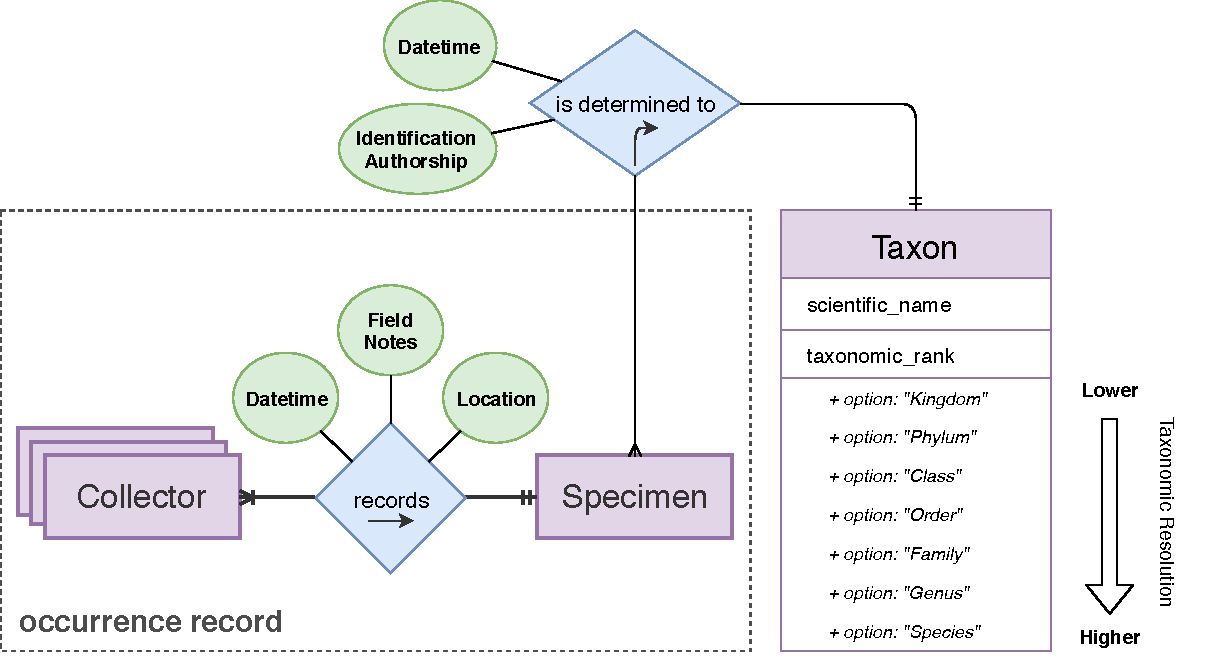
\includegraphics[width=\linewidth]{figures/collections_data/occurrences_er.pdf}
    \caption{Entity-relationship diagram illustrating the main features of occurrence records. The cardinality of relationships is represented using the Crow's foot notation.}
    \label{fig:occurrences_er}
\end{figure}

% Sources of occurrence data
%% Biological collections
In biological collections, specimens are physically stored in the collections, becoming vouchers that can be further referred to for a multitude of purposes, including for verifying their taxonomic identity.
Once a record is properly handled and deposited in the collection, the taxonomic identity of the collected specimen can be determined by professional taxonomists and incorporated to the original record. 
During this process the specimen is assigned to a single taxon, at the highest taxonomic resolution as possible.
%% Informal
Although biological collections are the major sources of occurrence data, occurrence data can be also gathered more informally by non-professional collectors.
A key difference, in this case, is that specimens are usually not physically collected. Thus, no vouchers are obtained.
This limits the application of this data in some contexts, but does not impact in others.
 e.g. citizen science and crowdsourcing projects.


Occurrence records are often recorded without random sampling, leading to biases in data.


%% Limitations and caveats % Graham2004-box3, Newbold2010
%%   - Stages in which we can have loss of data quality Chapman2005 intro
Distinct aspects of data quality can be affected in multiple stages of its life cycle \cite{Chapman2005}, including the moment of the recording event, its preparation before it can be deposited, the taxonomic determination, data digitization, data storage and analysis.
%%   - Biases: collector bias, taxonomic bias, (geographic bias, trait bias, historical bias, seasonal bias) % Daru2017, Haripersaud2009, [Kadmon, R., O. Farber, and A. Danin. 2004. Effect of roadside bias on the accuracy of predictive maps produced by bioclimatic models] [Schulman2007 (collecting bias)->  A mechanism for spatially characterizing collecting bias using Thiessen polygons] 
%%   - Errors:

%%   - Presence/absence data:

 


% Data issues
Although information about the occurrence of specimen in regions is turning massive and freely available, users of such data must be aware of some inherent caveats, coming from how the context in which data was recorded. 
Not all questions can be readily answered with such data, as there might be taxonomic, spatial,... biases.



% Citizen Science projects
% Data from citizen science projects are structured similarly, with a few differences: (i) absence of vouchered specimens; (ii) taxonomic determinations result from a collaborative community, not necessarily composed of specialists. 


% Data Aggregators
Gbif provides a data preprocessing routine % https://www.gbif.org/infrastructure/processing



% Biological collections data coverage and completeness \cite{Funk1999}.
% Completeness: How much of data representing the real distribution of a species has actually been collected?
% \cite{Jacobs2017}
% Completeness of biodiversity databases \cite{Soberon2007}


% Describing and publishing digitized datasets
% Data description (metadata).
% Data publication (Darwin Core).


%% As it is common practice for botanists to record each species once during field work, some important ecological attributes such as the species abundance are not to be directly inferred from such data. {check van Gemerden 2005, from Haripersaud2009}


% Biological collections are composed of aggregates of multiple biodiversity surveys, each recorded with particular methodologies
% Records sampled using distinct methodologies can be combined for optimizing data use \cite{VanGemerden2005}.

% Limitations in NHM data \cite{Graham2004 box3}
% Errors
% Biases
% Presence vc presence-absence data





% Data acquisition: (1) New collecting expeditions; (2) Collections exchanges materials with other institutions




% ============
% Data quality
% ------------
% [Soberon2004]

% Data quality among collection records is uneven -> worse for large datasets and for datasets composed by multiple sources
% Procedures are needed for correcting problems

% Quality issues: 
%% Determination issues: many specimens are incorrectly identified;
%% outdated taxonomy;
%% georreferencing errors.

% Data atomicity issues:
% Some fields are not atomic: more than one entity is represented as a single data element. 
% In the recordedBy field, Darwin Core standards state that distinct names should be separated by | (delimiter).
% This varies depending on the standard a collection uses. For example, the BRAHMS system recommends using a ';' as the delimiter.
% BRAHMS docs: https://herbaria.plants.ox.ac.uk/bol/brahms/support/documentation

% Identity issues:
% Entities are not guaranteed to have the same ids through distinct datasets.
% Even in the same datasets there may be variations in their names
% this is specially problematic for fields like the collectors field, which is overlooked for most applications of such data. 
% Some standards provide guidelines for including collectors names: last name + first initials...
% However different standards give distinct guidelines and thus name variants are common.
% How to map all name variants to the same entity? -> This leads to the Entity-resolution problem
Some common issues are: (i) including only the name of the first author of the occurrence, and eventually et.al grouping all other collectors;
(ii) format inconsistences when including multiple collectors. Some datasets do not use unique delimiter characters for separating collectors names, and thus affects the process of names atomization.
(iii) As collectors names are usually included in the form of last name followed by first initials, there are many cases of homonymous, especially for very common surnames (e.g. silva, souza,...).
There are also heteronymous, when distinct names variants are assigned to the same person. It can happen that two people have the same last name and their initials are the same (e.g. André Machado Souza or Ana Maria Souza leads to A.M.Souza).
This can also be the result of typos (e.g. souza becoming souza), or simply omiting parts of the name (e.g. if there are two collectors, A.M.Souza and A.P.Souza, omitting the middle initial makes their names indistinguishable).

% Data fit for use

In order to make data fit for its intended use the analyst must perform data cleaning.

% =============
% Data cleaning
% -------------
%[Chapman2005a]

% Why do we need data cleaning? -> We must make data fit for its indended use

% Goal: improving data quality, removing or treating entries that are 

% Adopting standardized collectors names
% Checking collectors itineraries -> look for the spatial pattern of records by the collector


% ================
% References
% ----------------
%% Museum-based informatics{Graham2004}









% Data Quality

% Preparing data 
% Data Selection
% Data Cleaning


% The Entity Resolution problem
\cite{Bhattacharya2007}

% Homonymous names, heteronymous names
% Typographic errors
First, using different naming conventions or occasionally including typographic errors while entering the data in the database leads to multiple variants of name.
Examples of typographic errors are mis
(such as names with typographic errors) homonymous names (a name
